\documentclass[12pt]{article}

\usepackage[margin=1in]{geometry}
\usepackage{amsmath,amsthm,amssymb}
\usepackage{mathrsfs}
\usepackage{mathtools}
\usepackage{enumitem}
\usepackage{physics}
\usepackage{pdfpages}

\newcommand{\magsq}[1]{\big|#1\big|^2}
\newcommand{\avg}[1]{\left<#1\right>}
\newcommand{\fullint}[1][x]{\int_{-\infty}^{\infty}\dd #1\;}
\newcommand{\halfint}[1][x]{\int_{0}^{\infty}\dd #1\;}

\begin{document}
	
\title{Homework 9}
\author{Sean Ericson \\ Phys 684}
\maketitle

\section*{Problem 1}
\subsection*{\small\underline{Problem}}
An atom has to recoil when emitting a photon. 
Calculate the velocity of a Na atom after the emission of a photon (assume that the atom is initially at rest and the optical transition takes place at the $\text{D}_2$ line with $\lambda = 589$ nm).
If we do not ignore the recoil energy, what will be the corresponding Doppler shift?

\subsection*{\small\underline{Solution}}
Using the calculations in the attached Mathematica notebook, we find that the resulting velocity is approximately 3 cm/s.
This motion produces a red shift in the wavelength of the light of approximately $5.8\times10^{-8}$ nm.

\section*{Problem 2}
\subsection*{\small\underline{Problem}}
For the $\text{D}_2$ transition of the Na atom, what is the Doppler cooling limit (assume $\gamma_2/2\pi=10$ MHz)?
What is the temperature limit of single photon recoil for the $\text{D}_2$ transition?

\subsection*{\small\underline{Solution}}
Using the calculations in the attached Mathematica notebook, we find that the Doppler cooling limit is $T_D \approx 120\;\mu$K. The temperature associated with a single recoil event is $T_R \approx 2.4\;\mu$K.


\section*{Problem 3 (Berman 5.2)}
\subsection*{\small\underline{Problem}}
Calculate the maximum force on an atom produced by a monochromatic, plane-wave field having Rabi frequency $\Omega_0/2\pi = 2   0$ MHz, given that $\gamma_2/2\pi = 10$ MHz and there are no collisions.
Assume that $v_z = 200$ m/s, that the resonance wavelength is $\lambda_0 = 628$ nm, and that the field can be tuned within 1 GHz of resonance.
Calculate the acceleration that this force produces for an atom having atomic mass 23.

\subsection*{\small\underline{Solution}}
Using the calculations in the attached Mathematica notebook, we find a maximum force of about 0.46 Attonewtons at a detuning of about 54.4 MHz.
Associated with this force is an acceleration of about 1.2$\times10^7$ m/$\text{s}^2$.


\section*{Problem 4 (Berman 5.3)}
\subsection*{\small\underline{Problem}}
For a 5-mW standing-wave laser field having a waist area of 4 $\text{mm}^2$, calculate the well depth of the ground-state potential produced by the field in units of the recoil energy $(\hbar^2k^2)/2M$ assuming a detuning of $3\gamma$.
Repeat the calculation for a FORT (Far Off-Resonance optical-dipole Trap), in which the laser field has a power of 100 mW and is focused to a spot diameter of 20 $\mu$m.
The detuning is 20$\gamma_2$. Take $\gamma_2/2\pi = 6$ MHz, $\lambda = 780$ nm, $M$ = \textsuperscript{85}Rb mass, and $\left(\mu_x\right)_{21} = -0.57ea_0$.
Also calculate the frequency spacing at the bottom of the wells assuming that the potentials can be approximated as harmonic in that region.
Can atoms cooled to the Doppler limit of laser cooling be trapped in these potentials? Explain.

\subsection*{\small\underline{Solution}}
Using the calculations in the attached Mathematica notebook, we find that the well depth for the 5-mW standing laser to be approximately 360 times the recoil energy.
For the 100-mW case, we find that the well depth is approximately 4.6$\times 10^7$ the recoil energy.
In both cases, the CoM energy associated with the Doppler cooling limit is several orders of magnitude smaller than the potential depth, so atoms cooled to the Doppler limit should indeed be trappable by these potentials.

The optical potential has the form
\[ V(z) = V_\text{opt}\sin(kz). \]
Near a minimum, this is approximated by
\[ V(z) \approx V_\text{opt}\left(\frac{(kz)^2}{2} - 1\right). \]
Ignoring the offset, we have that
\begin{alignat*}{3}
    &\quad & V &\sim \frac{1}{2}V_\text{opt}k^2z^2 \\
    & & &= \frac{1}{2}m\tilde{\omega}^2z^2 \\
    &\implies & \tilde{\omega} &= \sqrt{\frac{V_\text{opt}k^2}{m}}
\end{alignat*}

Using the the given values, we find that the potentials produce frequency spacings of $\tilde{\omega} \approx $ 0.1 MHz and 37 MHz, respectively.


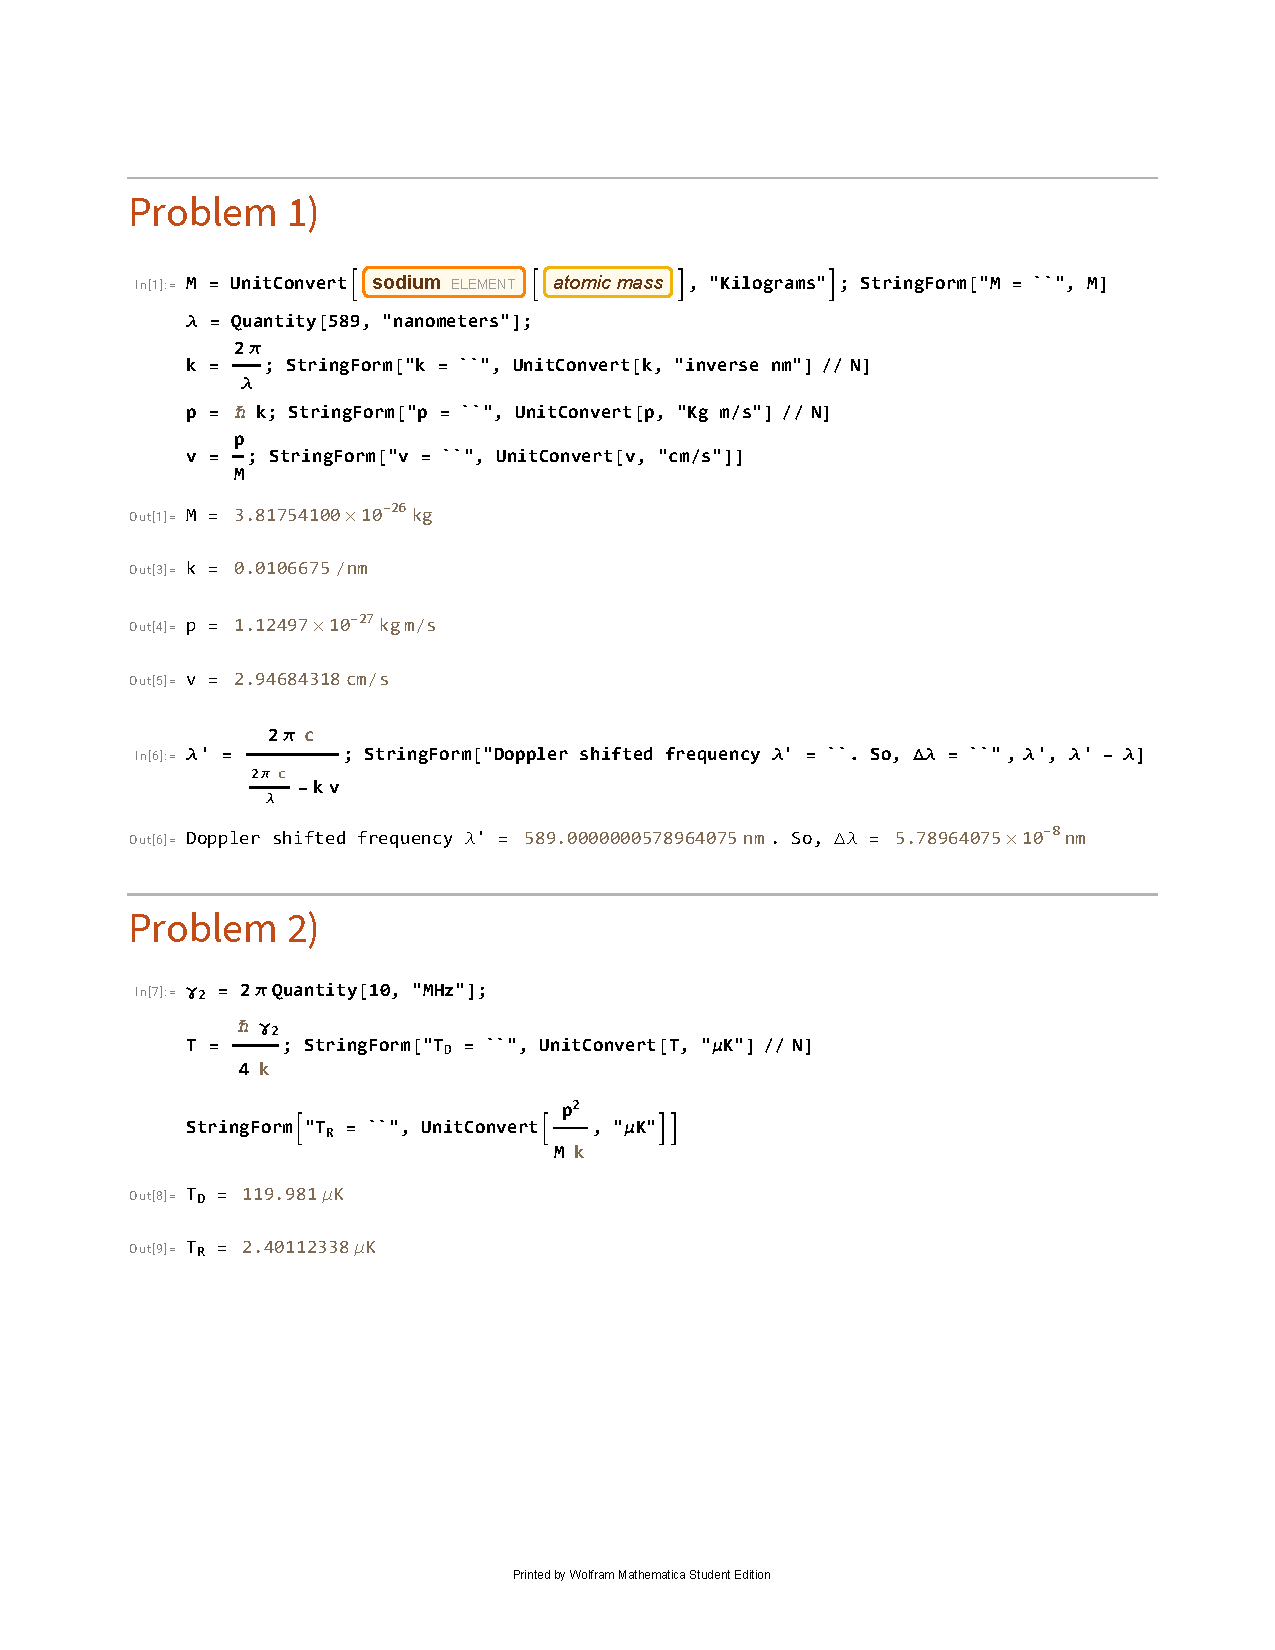
\includepdf[pages=-]{calcs/hw_9.pdf}
\end{document}